\documentclass[11pt]{article}
  \usepackage[utf8]{inputenc}
  \usepackage{graphicx}
\title{Relazione Progetto Programmazione ad Oggetti 2014/2015}
\author{Suierica Bogdan Ionut 1008089}

\begin{document}
	\maketitle
	\begin{figure}[h]
\centering
\includegraphics[width=0.7\linewidth]{../../../Dropbox/touslesmemes/RelazioneExtra/img/unipd}

\end{figure}

	\newpage
	\section{Introduzione}
		\subsection{Scopo del documento}
		Lo scopo del documento è quello di presentare le principali scelte architetturali del progetto.
		\subsection{Scopo del progetto}
		Lo scopo del progetto è lo sviluppo in C++/Qt di un sistema minimale per l'amministrazione ed utilizzo tramite interfaccia utente grafica di un (piccolo) database di contatti professionali ispirato a Linkedin.
		\subsection{Specifiche progettuali}
		Il progetto è stato sviluppato in un sistema Mac Os X Yosemite. Nello sviluppo è stato utilizzato l'ide Qt Creator versione 3.3.0 con versione delle librerie 5.4.4. Il tool Qt Designer non è stato utilizzato nello sviluppo delle interfacce grafiche ma solo per avere un riferimento grafico. \\Il progetto è stato provato sui computer del laboratorio in Paolotti e compila ed esegue correttamente.\\
		Il programma consente di aprire e salvare il database in formato XML. L'apertura e il salvataggio del database avvengono in automatico in quanto il path è di default. \\
		Nel progetto ho cercato di dividere il più possibile la parte logica dalla parte grafica.
		\newpage
		
	\section{Classi logiche}
	Ho sviluppato una gerarchia da 4 classi: 
	\begin{figure}[h]
\centering
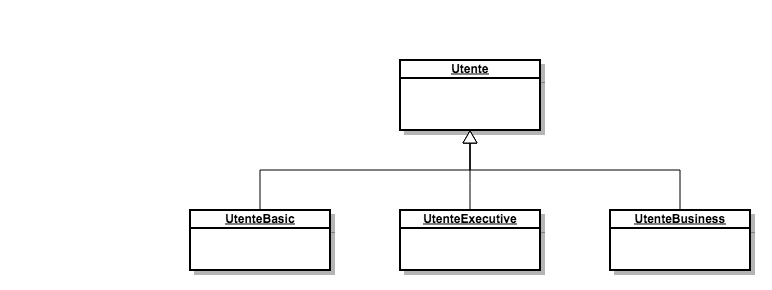
\includegraphics[width=0.8\linewidth]{gerarchiaUtente}
\caption{Gerarchia Utenti}
\label{fig:Gerarchia Utente}
	\end{figure}
	
	La classe base è la classe \textit{Utente} e rappresenta un utente LinQedIn generico. Per questo motivo si è scelto di rendere questa classe astratta e quindi non è possibile dichiarare oggetti di questo tipo. Non avedo a disposizione metodi virtuali puri è stato scelto di rendere il distruttore virtuale puro.\\
	Le classi \textit{UtenteBasic}, \textit{UtenteExecutive} e \textit{UtenteBusiness} sono classi concrete derivate direttamente dalla classe base \textit{Utente}. \\
	La classe \textit{Rete} raffigura la relazione di amicizia ed è rappresentata dal username del contatto. \\
	La classe \textit{InfoPersonali} è rappresentata da un nome, cognome, anno di nascita e una descrizione dell'utente. \\
	La classe \textit{Profilo} rappresenta il profilo di un utente ed è stato scelto di rappresentarla come vector di puntatori a \textit{Competenze}, \textit{Esperienze}, \textit{Formazione}, \textit{Lingue}.
	\begin{itemize}
		\item Classe Competenze: raffigura le competenze di un utente ed è rappresentata dal nome della competenza e il voto che può essere espresso con un numero compreso tra 1 e 10, dove 1 è il minimo e 10 e il massimo;
		\item Classe Esperienze: raffigura le esperienze nel campo lavorativo del utente ed è rappresentata dal nome dell'azienda in cui ha lavorato e il periodo tra il quale ha lavorato;
		\item Classe Formazione: con formazione si intendono tutti i diplomi acquisiti in seguito a un percorso di studio. La classe è rappresentata dal nome del ramo/indirizzo/facoltà e dall'anno conseguimento diploma;
		\item Classe Lingua: raffigura le lingue studiate dal utente. La classe è rappresentata dal nome della lingua e il livello di conoscenza della lingua:
		\begin{itemize}
			\item Basic;
			\item Avanzato;
			\item Eccelente;
			\item Madre Lingua;
		\end{itemize}
	\end{itemize}
	L'utente è caratterizzato da:
	\begin{itemize}
		\item Username: univoco;
		\item Informazioni Personali: rappresentato tramite un puntatore alla classe \textit{InfoPresonali};
		\item Profilo: rappresentato tramite un puntatore alla classe \textit{Profilo};
		\item Rete di contatti: rappresentato tramite un vector di puntatori alla classe \textit{Rete}. È presente il distruttore profondo.
	\end{itemize}
	La classe \textit{DB} è la classe collezione utenti ed è stato scelto di rappresentarla tramite un vector di puntatori a \textit{Utente} sfruttando l'ereditarietà. La classe \textit{DB} contiene anche un distruttore profondo e metodi di aggiunta e rimozione dei singoli elementi. Per gestire il contenuto del database su un file \textit{XML} sono state utilizzate le seguenti classi offerte da Qt:
	\begin{itemize}
		\item QDomDocument;
		\item QXmlStreamWriter.
	\end{itemize}
	Come contenitori ho scelto di usare i vector in quanto l'inserimento viene fatto sempre in coda in tempo O(1). Gli oggetti dei vector vengono allocati esclusivamente sullo heap.
	\subsection{Ricerca}
	La funzionalità di ricerca cambia in funzione alla propria tipologia di account. Le tre tipologie di account descritte sopra permettono delle funzionalità di ricerca crescenti:
	\begin{itemize}
		\item Basic permette una ricerca che controlla solamente se esiste l'utente. Ritorna il nome, cognome e l'anno di nascita;
		\item Business permette una ricerca che ritorna tutte le informazioni di un utente meno i contatti dell'utente ricercato;
		\item Executive permette una ricerca completa.
	\end{itemize}
	La ricerca è stata implementata attraverso i funtori ed è stato utilizzato come riferimento lo scheletro logico con funtori offerto dal Prof. Ranzato.
	\section{Classi grafiche}
	La classe \textit{MainWindow} è la finestra principale del programma. Alla sua creazione viene costruito anche l'oggetto \textit{DB} che contiene il database degli utenti. Qui è possibile selezionare la modalità in cui si vuole accedere, utente o amministratore.
	\begin{figure}[h]
\centering
\includegraphics[width=0.6\linewidth]{../../../Desktop/main}
\caption[Finestra principale]{Finestra principale}
\label{fig:main}
	\end{figure}
	
	\newpage
	La classe \textit{ClientWindow} è la finestra destinata agli utenti del servizio. Qui si può modificare il proprio profilo e ricercare altri utenti. È stato scelto la derivazione da \textit{QDialog} per fare in modo che sia una finestra bloccante e non possa interagire con altre finestre del programma finché non sarà chiusa. 
	\begin{figure}[h]
\centering
\includegraphics[width=0.6\linewidth]{../../../Desktop/client}
\caption[Finestra utente]{Finestra utente}
\label{fig:client}
\end{figure}


	La classe \textit{AdminWindow} è la finestra destinata all'amministratore. Qui è possibile aggiungere un nuovo utente, selezionare un utente e cambiare la tipologia di account tra basic, executive e business cosi come la rimozione o la ricerca di un utente. È stato scelto la derivazione da \textit{QDialog} per fare in modo che sia una finestra bloccante e non possa interagire con altre finestre del programma finché non sarà chiusa.
		\begin{figure}[h]
			\centering
			\includegraphics[width=0.5\linewidth]{../../../Desktop/admin}
			\caption[Finestra amministrazione]{Finestra amministrazione}
			\label{fig:admin}
		\end{figure}
		\newpage
		La ricerca e l'autenticazione viene fatta tramite username. Al momento del autenticazione e della ricerca viene effettuato un controllo sulla presenza o meno del username. Nel caso in cui l'username non fosse presente, viene visualizzato un messaggio di errore.

		\section{Gestione della memoria}
		Nel progetto gli oggetti di tipo \textit{Utente} e derivati da \textit{Utente}, \textit{Profilo}, \textit{InfoPersonali}, \textit{Rete} sono allocati esclusivamente sullo heap. Sono stati ridefiniti i distruttori e quindi le classi sono fornite di un distruttore profondo che permette la deallocazione degli oggetti dallo heap nel momento in cui viene distrutto il puntatore.
		Se l'utente decide di chiudere tutte le finestre viene eseguita un'operazione di svuotamento dei vector che prima dealloca gli oggetti puntati dai puntatori e poi rimuove tutti gli elementi del vector.

\end{document}